\newpage
	\section{\Large ZIELBESTIMMUNG}
	\begin{itemize}
		\item Korrektheit der Nodes
		\item Struktur
		\item Benutzerfreundlichkeit
	\end{itemize}
	\subsection{Musskriterien}
	\begin{itemize}
		\item Das System muss auf dem Kartenbezugssystem WGS 84 laufen
		\item Das System muss nach Eingabe von Breiten- \& Längengrad eine Teilkarte ausgeben. Auf dieser Karte sind die Bundesautobahnen und Bundesstraßen sowie Richtungspfeile in die, die Autobahn/Straße verläuft, eingezeichnet. Dabei zeigen die Pfeile in die jeweilige Richtung der nächsten Node.
		\item Das System muss die Pfeil-Nodes, so anpassen das z.b. Geschwindigkeitsbeschränkungen gespeichert werden können.
		\item Das System muss nach Eingabe einer minimalen und maximalen-Eingabe eines Punktes. Den Ausschnitt der Karte darstellen.
		\item Das System muss nachdem eine Karte dargestellt wurde, den ausgewählten Kartenbereich verschieben können.
		\item Das System muss skalierbar sein.
	\end{itemize}
	\subsection{Abgrenzungskriterien}
	\begin{itemize}
		\item Das System ist keine Navigations Software
		\item Das System zeigt keine genauen Karten Informationen an
	\end{itemize}
	
	
	\section{\Large PRODUKTEINSATZ}
	\subsection{Anwendungsbereiche}
	\begin{itemize}
		\item Das Produkt soll im privaten Bereich eines Benutzers Anwendung finden.\\
		Es soll nicht für gewerbliche Zwecke oder für Anbahnung von Geschäften genutzt werden.
	\end{itemize}
	\subsection{Zielgruppen}
	\begin{itemize}
		\item Die Zielgruppe sind Leute, 
		\begin{itemize}
			\item die Wert auf \textbf{"Wege zur Gewinnung und Korrektur von Kartendaten"} legen.
			\item die Initiativen für \textbf{"GeoInformation und Navigation"} unterstützen.
		\end{itemize}
	\end{itemize}
	\subsection{Betriebsbedingungen}
	\begin{itemize}
		\item Das Produkt benötigt eine stetige Internetverbindung und den Dienst der die *.OSM Dateien zur Verfügung stellt. Unser Service wird angeboten solange wir Zugriff auf die *.OSM Dateien haben.
	\end{itemize}
	
	
	\section{\Large PRODUKTÜBERSICHT}
	Gibt eine Übersicht über das Produkt, z.B. über alle wichtigen Geschäftsprozesse in Form eines Übersichtsdiagramms.
	\subsection{Usecase Diagramm}
		\begin{figure}[H]
			\centering
			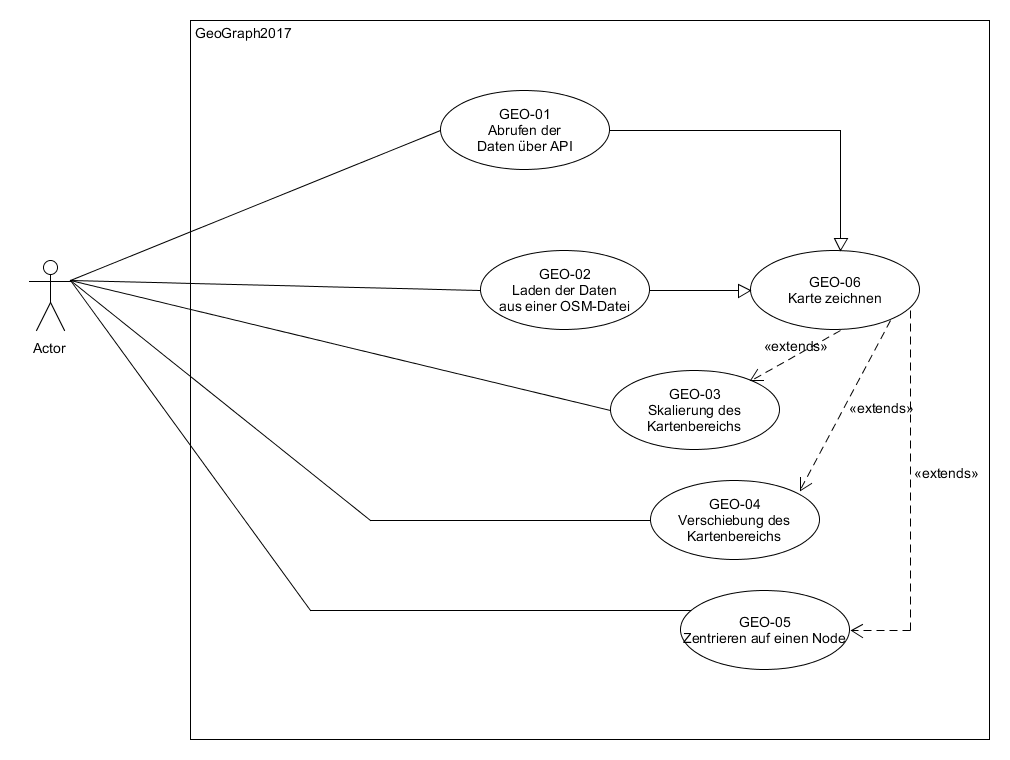
\includegraphics[width=0.7\linewidth]{images/Usecases}
			\caption{}
			\label{fig:GUI}
		\end{figure}
		
		
	\section{\Large PRODUKTFUNKTIONEN}
	\subsection{Usecase-Beschreibungen}

	\begin{table}[H]
		\begin{tabular}{|p{8cm}|p{8cm}|}
			\hline
			\textbf{GEO-01 } \\ 
			\hline
			\textbf{ID :}\centering & GEO-01  \\ \hline 
			\textbf{Title :}\centering & Abruf der Daten über API \\ \hline 
			\textbf{Description :}\centering & Daten für die Karte werden per API abgerufen \\ \hline 
			\textbf{Trigger :}\centering & User klickt auf den Button "Nach Koordinaten suchen" \\ \hline 
			\textbf{Primary Actor :} \centering & User \\ \hline 
			\textbf{Preconditions :}\centering & 
			1. Programm ist gestartet \newline 
			2. User hat Längen und Breitengrad eingegeben	\\ \hline 
			\textbf{Postconditions :}\centering &  
			1. User hat den Kartenbereich erfolgreich geladen \newline 
			2. Karte wird angezeigt \\ \hline
			\textbf{Other Use Cases :}\centering & - \\ \hline  
			\textbf{Main Success Scenario :}\centering & 
			1. User gibt Längen und Breitengrad ein \newline
			2. User klickt auf "Nach Kordinaten suchen" \newline
			3. Karte wird angezeigt \\ \hline  
			\textbf{Extensions :}\centering & - \\ \hline  
			\textbf{Priority :}\centering & High \\ \hline  
		\end{tabular}
	\end{table}
	
	\begin{table}[H]
		\begin{tabular}{|p{8cm}|p{8cm}|}
			\hline
			\textbf{GEO-02 } \\ 
			\hline
			\textbf{ID :}\centering & GEO-02  \\ \hline 
			\textbf{Title :}\centering & Laden der Daten aus einer OSM-Datei \\ \hline 
			\textbf{Description :}\centering & Daten für die Karte werden aus der hinterlegten OSM-Datei geladen \\ \hline 
			\textbf{Trigger :}\centering & User klickt auf den Button "Nach Koordinaten suchen" \\ \hline 
			\textbf{Primary Actor :} \centering & User \\ \hline 
			\textbf{Preconditions :}\centering & 
			1. GEO-01\\ \hline 
			\textbf{Postconditions :}\centering & 
			1. User hat Kartenbereich aus OSM-Datei geladen \newline
			2. Karte wird angezeigt \\ \hline
			\textbf{Other Use Cases :}\centering & - \\ \hline  
			\textbf{Main Success Scenario :}\centering & 
			1. GEO-01 \newline
			2. User klickt auf " Nach Kordinaten suchen" \newline
			3. Karte wird angezeigt \\ \hline  
			\textbf{Extensions :}\centering & - \\ \hline  
			\textbf{Priority :}\centering & High \\ \hline  
		\end{tabular}
	\end{table}
	
	\begin{table}[H]
		\begin{tabular}{|p{8cm}|p{8cm}|}
			\hline
			\textbf{GEO-03 } \\ 
			\hline
			\textbf{ID :}\centering & GEO-03  \\ \hline 
			\textbf{Title :}\centering & Skalierung des Kartenbereichs  \\ \hline 
			\textbf{Description :}\centering & Skaliert den Kartenbereich via Regler  \\ \hline 
			\textbf{Trigger :}\centering & User bewegt den Slider in den positiven/negativen Bereich  \\ \hline 
			\textbf{Primary Actor :} \centering & User \\ \hline 
			\textbf{Preconditions :}\centering & 
			1. User hat GEO-01 oder GEO-02 ausgeführt \\ \hline 
			\textbf{Postconditions :}\centering & 
			1. User bewegt Slider in den positiven/negativen Bereich \newline
			2. Kartenausschnitt vergrößert/verkleinert sich \newline
			3. Karte wird angezeigt \\ \hline
			\textbf{Other Use Cases :}\centering & - \\ \hline  
			\textbf{Main Success Scenario :}\centering & 
			1. GEO-01 oder GEO-02 \newline
			2. User bewegt Slider in Positiven/Negativen Bereich \newline
			3. Karte wird vergrößert/verkleinert \newline
			4. Karte wird angezeigt \\ \hline  
			\textbf{Extensions :}\centering & - \\ \hline  
			\textbf{Priority :}\centering & High \\ \hline  
		\end{tabular}
	\end{table}
	
	\begin{table}[H]
		\begin{tabular}{|p{8cm}|p{8cm}|}
			\hline
			\textbf{GEO-04 } \\ 
			\hline
			\textbf{ID :}\centering & GEO-04  \\ \hline 
			\textbf{Title :}\centering & Verschiebung des Kartenbereichs \\ \hline 
			\textbf{Description :}\centering & Verschiebt den Kartenbereich via Maus \\ \hline 
			\textbf{Trigger :}\centering & User bewegt die Maus in den Kartenausschnitt und hält die linke Maustaste gedrückt und schiebt dann in x/y Richtung  \\ \hline 
			\textbf{Primary Actor :} \centering & User \\ \hline 
			\textbf{Preconditions :}\centering & 
			1. GEO-01 oder GEO-02 \\ \hline 
			\textbf{Postconditions :}\centering & 
			1. User bewegt die Maus in x/y Richtung \newline
			2. Der Kartenausschnitt bewegt sich in x/y Richtung \newline
			3. Der Kartenausschnitt wird angezeigt \\ \hline
			\textbf{Other Use Cases :}\centering & - \\ \hline  
			\textbf{Main Success Scenario :}\centering & 
			1. GEO-01 oder GEO-02 \newline
			2. User hält Maus gedrückt und schiebt den Kartenausschnitt \newline
			3. Kartenausschnitt wird angezeigt \\ \hline  
			\textbf{Extensions :}\centering & 
			1. Nur zuvor geladener Kartenausschnitt wird angezeigt \\ \hline  
			\textbf{Priority :}\centering & High \\ \hline  
		\end{tabular}
	\end{table}
	
	\begin{table}[H]
		\begin{tabular}{|p{8cm}|p{8cm}|}
			\hline
			\textbf{GEO-05 } \\ 
			\hline
			\textbf{ID :}\centering & GEO-05  \\ \hline 
			\textbf{Title :}\centering & Zentrierung auf einer Node \\ \hline 
			\textbf{Description :}\centering & Zentrierung auf einer Node nach eingabe von Langen-und Breitengrad \\ \hline 
			\textbf{Trigger :}\centering & User gibt Breiten-und Längengrad ein und die nächstgelegende Node wird zentriert \\ \hline 
			\textbf{Primary Actor :} \centering & User \\ \hline 
			\textbf{Preconditions :}\centering & 
			1. GEO-01 oder GEO-02 \\ \hline 
			\textbf{Postconditions :}\centering &
			1. Kartenausschnitt wird auf die nächstgelgende Node verschoben \newline
			2. Karte wird auf die Node zentriert \newline
			3. Karte wird angezeigt \\ \hline
			\textbf{Other Use Cases :}\centering & - \\ \hline  
			\textbf{Main Success Scenario :}\centering &
			1. GEO-01 oder GEO-02 \newline
			2. Kartenausschnitt wird verschoben \newline
			3. Karte wird auf Node zentriert \newline
			4. Karte wird angezeigt \\ \hline  
			\textbf{Extensions :}\centering & - \\ \hline  
			\textbf{Priority :}\centering & High \\ \hline  
		\end{tabular}
	\end{table}	
	
	\subsection{Aktivitätsdiagramm}
		\begin{figure}[H]
			\centering
			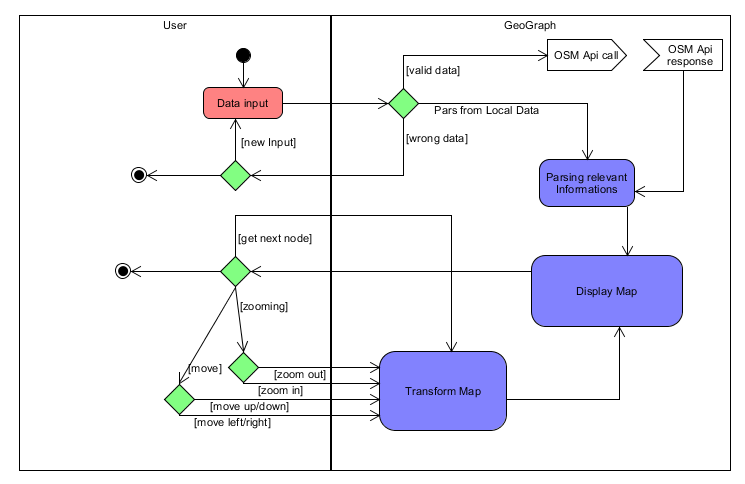
\includegraphics[width=0.7\linewidth]{images/Ablauf}
			\caption{}
			\label{fig:Akitiviti}
		\end{figure}
	\subsection{Sequenzdiagramm}
	\begin{figure}[H]
	\centering
	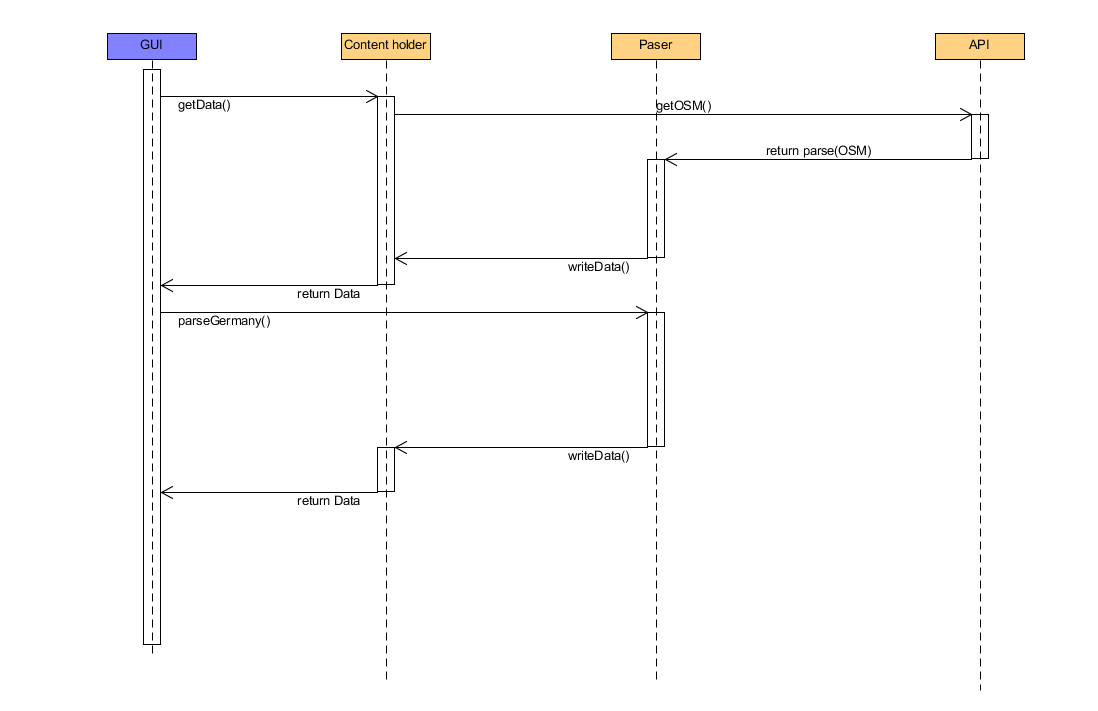
\includegraphics[width=0.7\linewidth]{images/Squenz}
	\caption{}
	\label{fig:Seq}
	\end{figure}
	
	
	\section{\Large PRODUKTDATEN}
		Langfristig sollen folgende Daten im System gespeichert | ausgelesen werden:
	\begin{itemize}
		\item Speicherung der Straßenpunkte als OSM-Datei
		\item Laden der Daten via Overpass API
	\end{itemize}
	\subsection{Analyseklassendiagramm}	
		\begin{figure}[H]
		\centering
		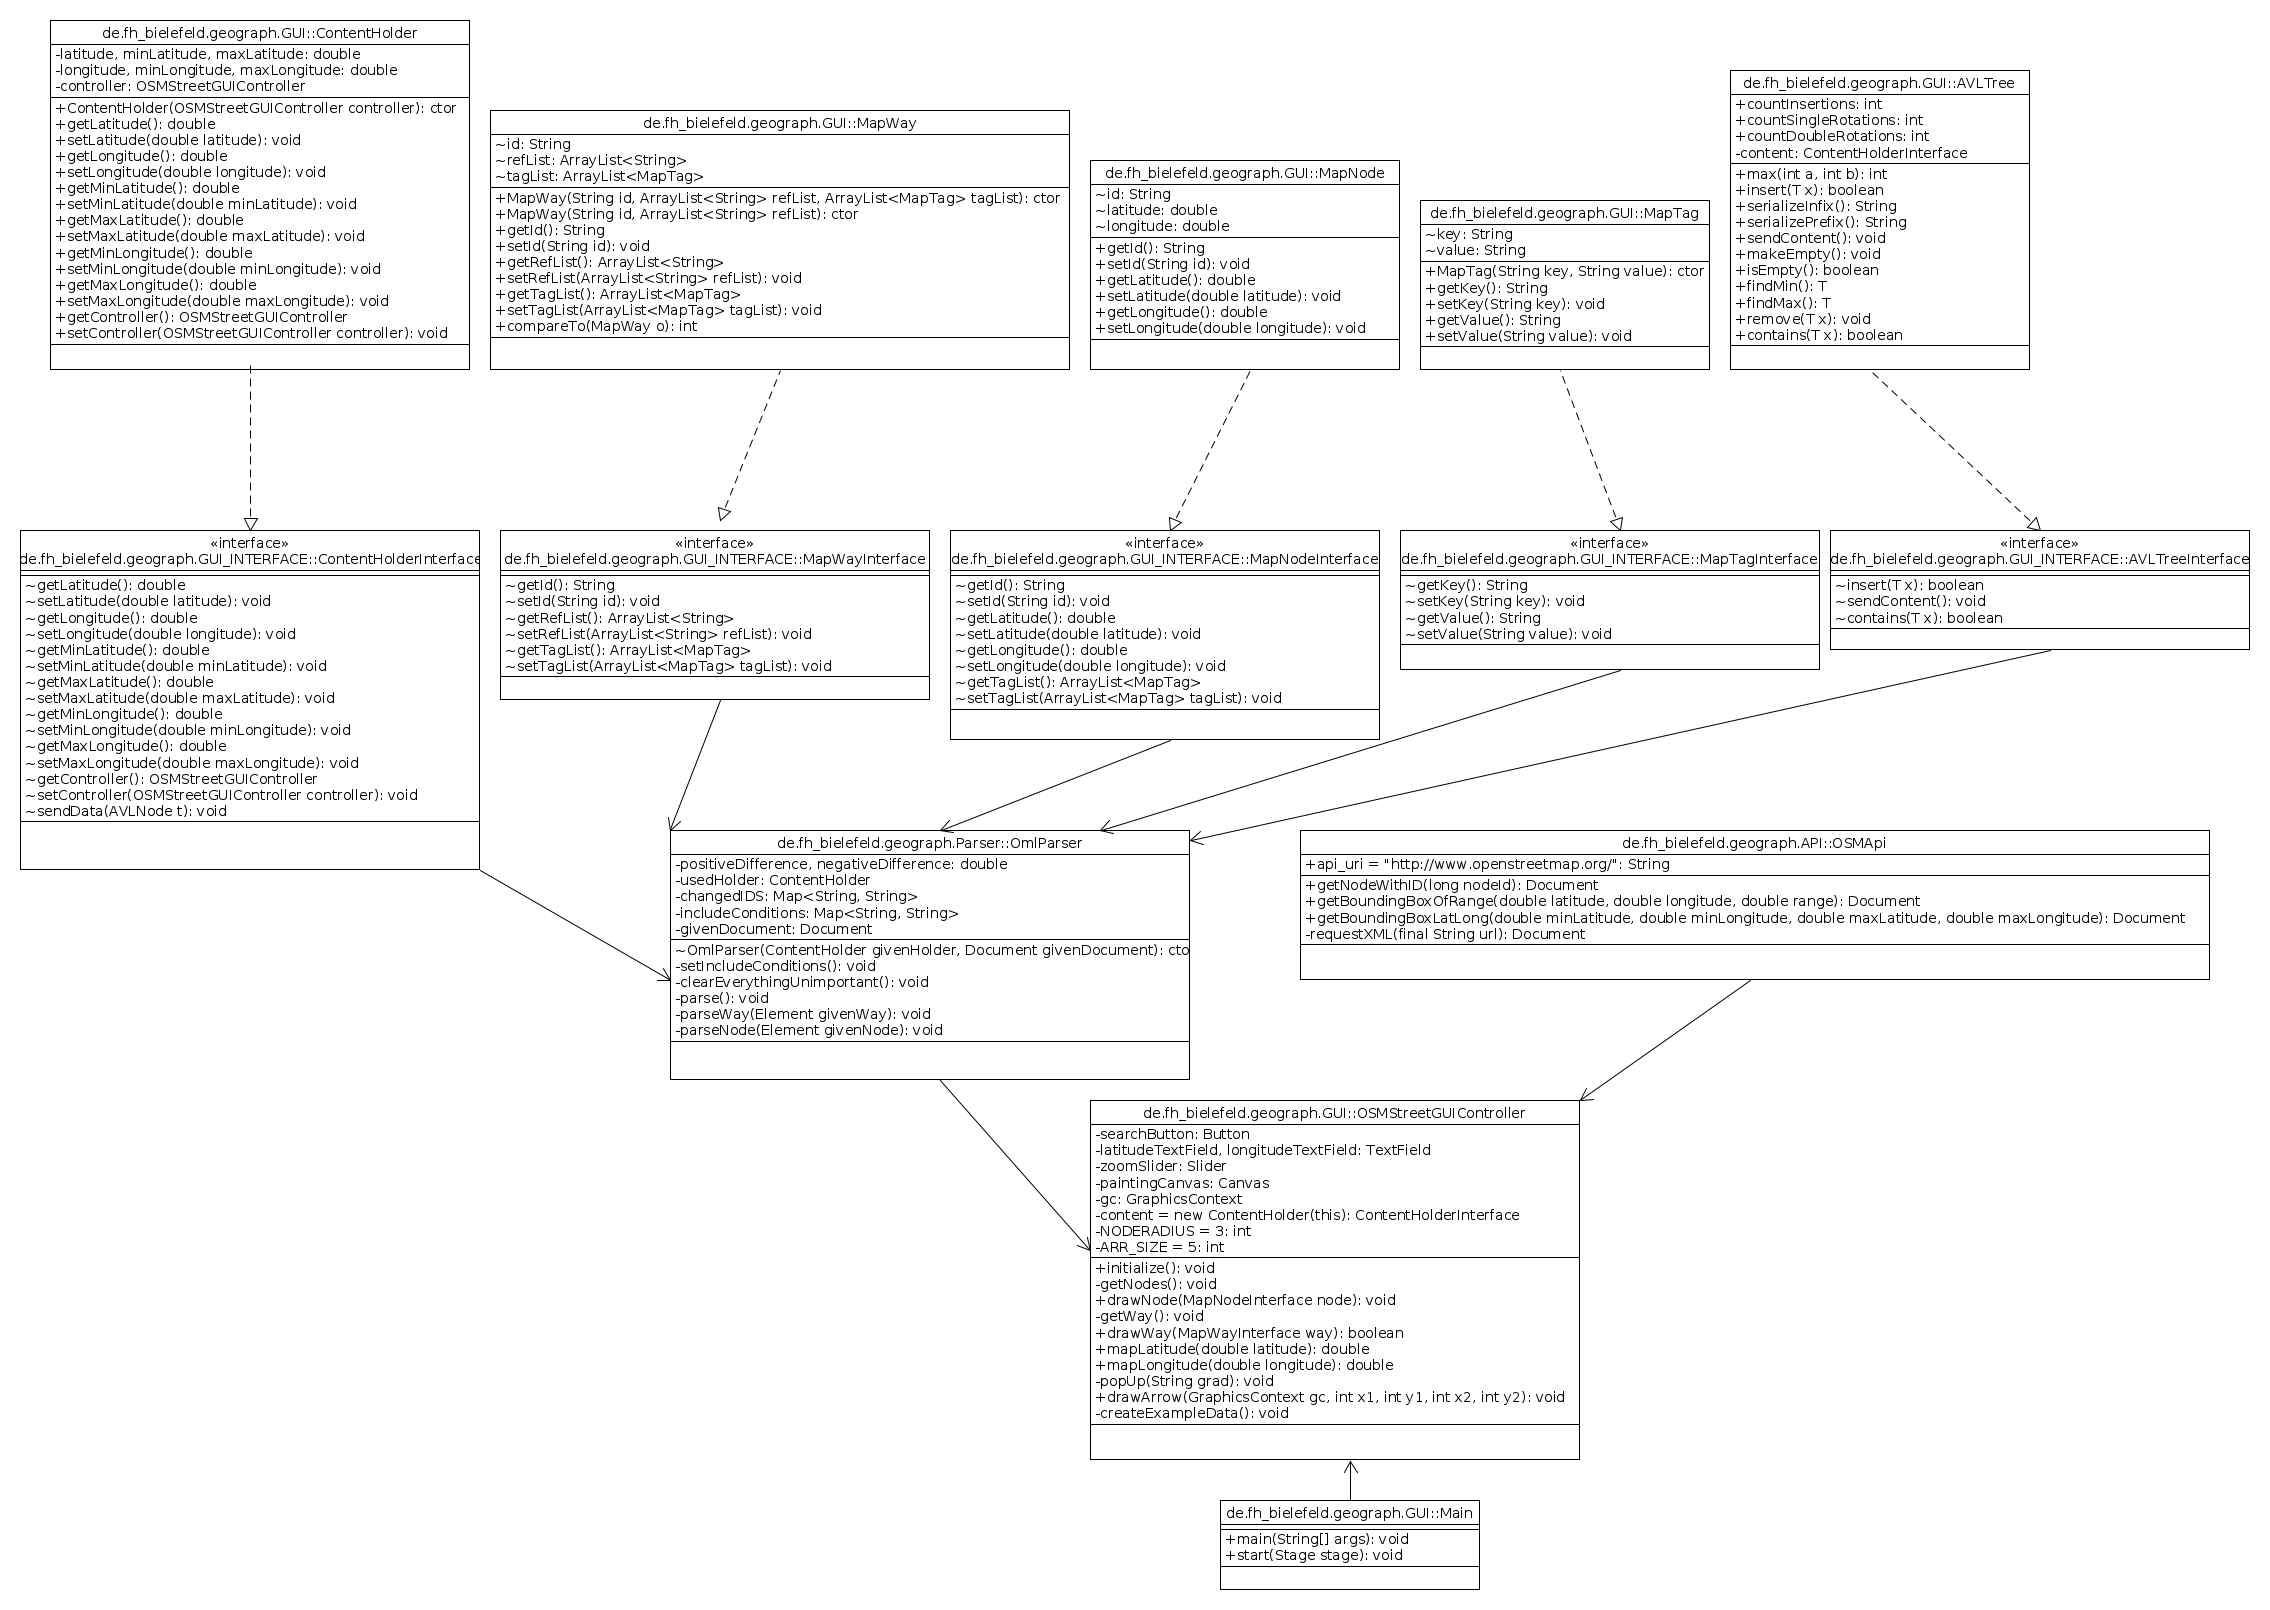
\includegraphics[width=0.7\linewidth]{images/Klassendiagramm}
		\caption{Klassendiagramm}
		\label{fig:Klassendiagramm}
	\end{figure}
	\subsection{Paketdiagramm}
		\begin{figure}[H]
			\centering
			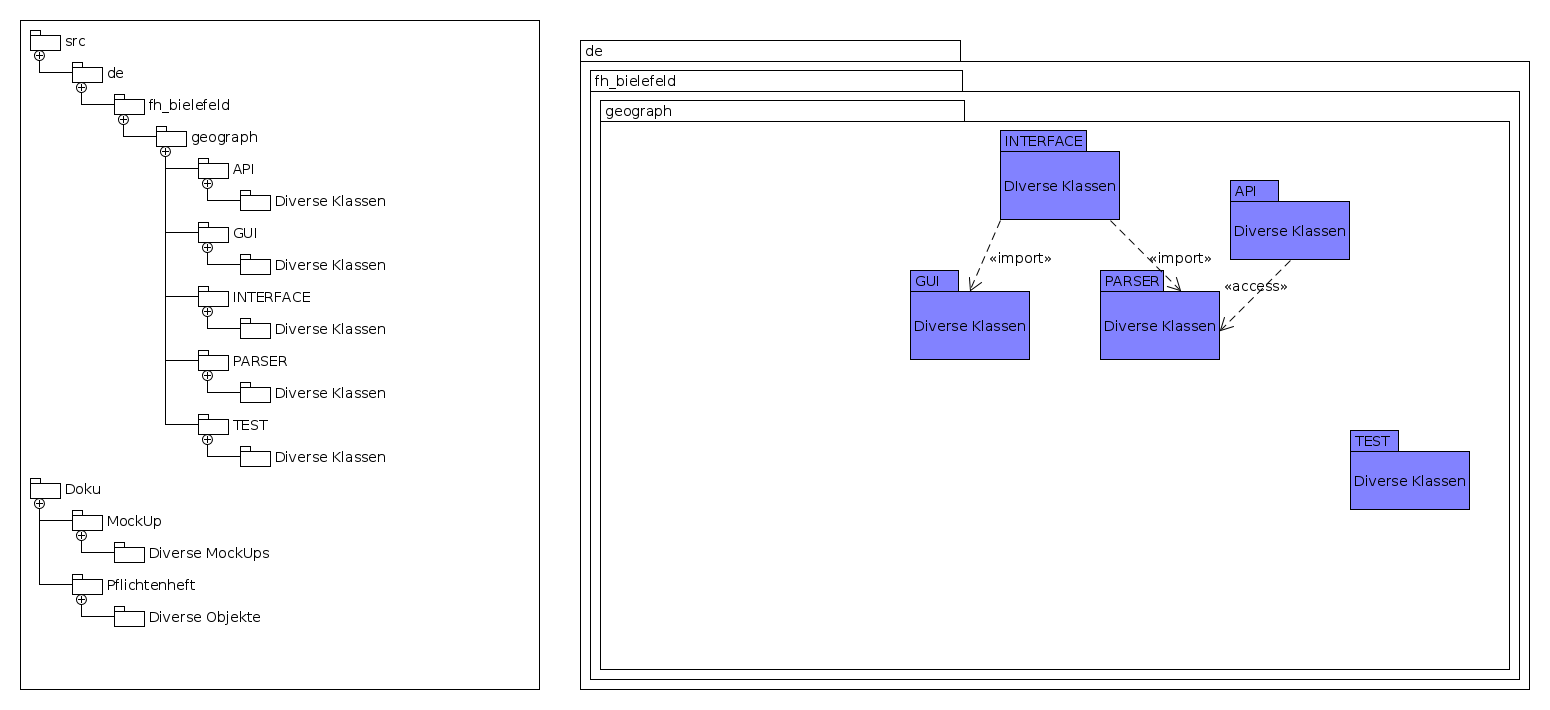
\includegraphics[width=0.7\linewidth]{images/Paketdiagramm}
			\caption{Paketdiagramm}
			\label{fig:Paketdiagramm}
		\end{figure}
	\subsection{Domänenklassendiagramm}
	\section{\Large PRODUKTLEISTUNGEN}
	\begin{itemize}
		\item Nicht genauer spezifiziert.
	\end{itemize} 
		
	
	\section{\Large QUALITÄTSANFORDERUNGEN}
	\begin{itemize}
		\item Nicht genauer spezifiziert.
	\end{itemize}
	
	\section{\Large BENUTZEROBERFLÄCHE}
	Es gibt eine Rolle und das ist die des Users der das Prgoramm ausführt (GUI).
	\begin{figure}[H]
	\centering
	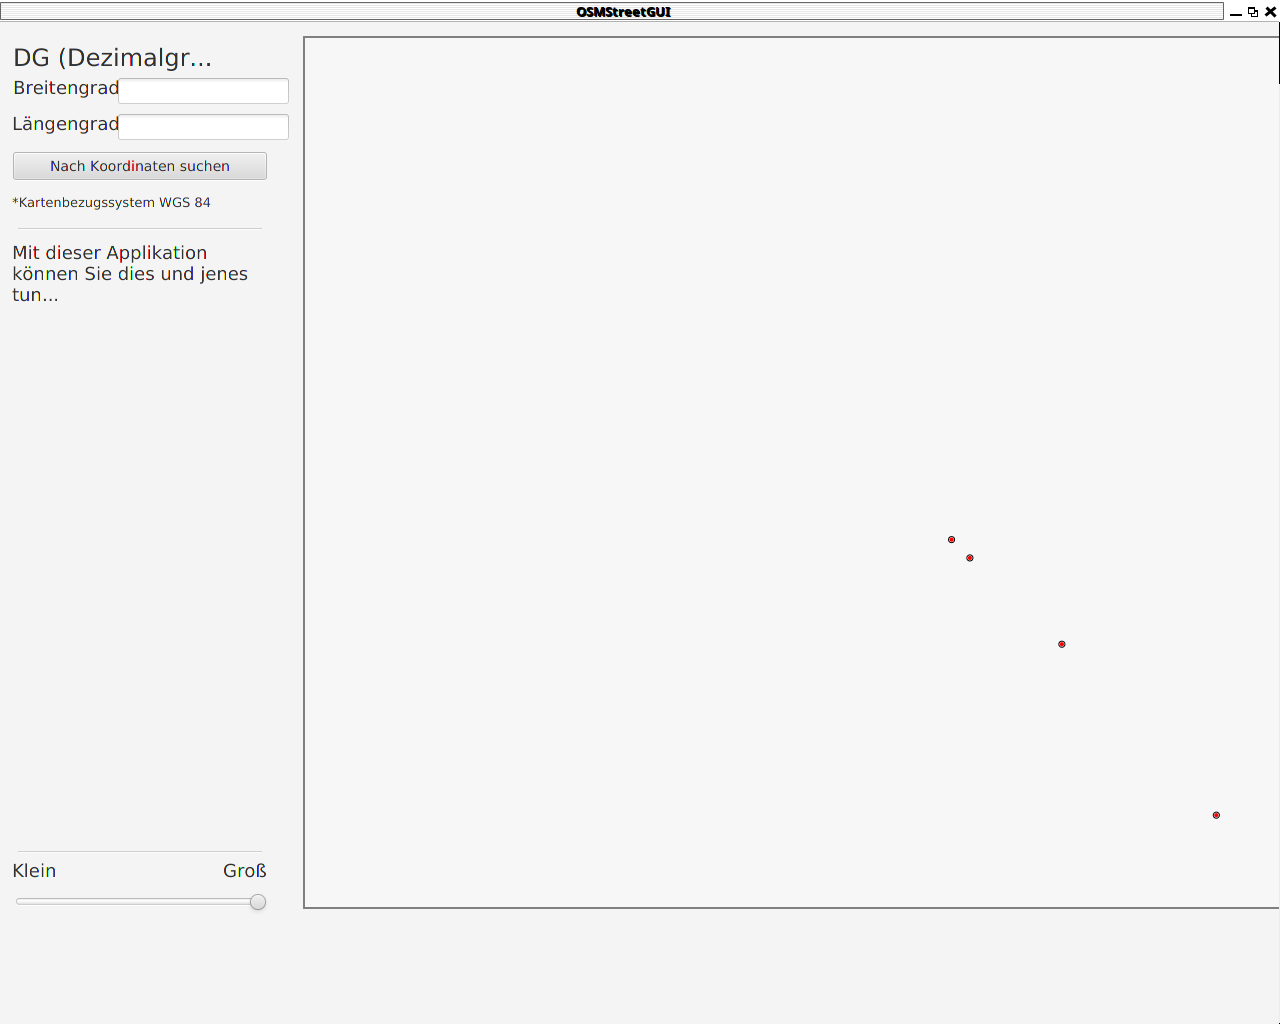
\includegraphics[width=0.7\linewidth]{images/GUI}
	\caption{}
	\label{fig:GUI}
	\end{figure}
	
	\subsection{Ansicht: verschiedene Ansichten 1 2 3 4 5}
	\subsection{Zusatandsdiagramme}
	\subsection{Ansicht: verschiedene Zustandsdiagramme 1 2 3 4 5}
	
	
	\section{\Large NICHTFUNKTIONALE ANFORDERUNGEN}
	Es werden alle Anforderungen aufgeführt, die sich nicht auf die Funktionalität, \textbf{ die Leistung} und \textbf{ die Benutzungsoberfläche} beziehen, z.B. :
	\begin{itemize}
		\item Einzuhaltende \textbf{Gesetze}
		\item Einzuhaltende \textbf{Normen}
		\item Testat durch externe Prüfungsgesellschaft
		Revisionsfähigkeit 
		\item Ordnungsmäßigkeit der Buchführung
		\item \textbf{ Sicherheitsanforderungen, z.B. :}
		\begin{itemize}
			\item Richtigkeit der Nodes
			\item Richtigkeit der Pfeile
			\item Genauigkeit der Nodes
			\item Genauigkeit der BoundingBox
			\item Genauigkeit beim Skalieren
		\end{itemize}  
		\item Plattformabhängigkeiten
		\item Sehr performant in Abhängigkeit zur Downloadgeschwindigkeit
		\item Aktuelle Betriebssysteme abdecken(Windows, Linux)
		\item Daten müssen gespeichert werden	 
	\end{itemize} 

	
	\section{\Large TECHNISCHE PRODUKTUMGEBUNG}
   	In diesem Kapitel wird die technische Umgebung des Produkts beschrieben.\\
   	Bei Client / Server-Anwendungen ist die Umgebung jeweils für Clients und Server getrennt anzugeben.
	\subsection{Software}
	\begin{itemize}
		\item Erfordert \textbf{Java} auf dem Client
		\begin{itemize}
			\item getestet und entworfen wird für :
			\begin{itemize}
				\item PC | Laptop
				\begin{itemize}
					\item Windows ab Version 7
					\item Linux
				\end{itemize}
			\end{itemize}
		\end{itemize}
	\end{itemize}
	\subsection{Hardware}
	\begin{itemize}
		\item \textbf{Internetfähiges Gerät :}
		\begin{itemize}
			\item PC | Laptop
			\item \textbf{Minimale Bildschirmauflösung :}
				\begin{itemize}
					\item 1024 x 768 Pixel Hochformat / Querformat
				\end{itemize}
					\item \textbf{Maximale Bildschirmauflösung :}
				\begin{itemize}
				\item 4096 × 2160 Pixel Hochformat / Querformat
				\end{itemize}		
		\end{itemize}
	\end{itemize}
	\subsection{Orgware}
	\begin{itemize}
		\item Der Client benötigt eine Internetverbindung.
		\item Um eine befriedigende Nutzererfahrung zu gewährleisten, werden folgende Bandbreiten-Untergrenzen definiert:
		\begin{itemize}
			\item \textbf{ PC | Laptop :}
			\begin{itemize}
				\item DSL Verbindung mit min. 2 Mbit/s Download-Bandbreite
			\end{itemize}
		\end{itemize}
	\end{itemize}
	\subsection{Produkt-Schnittstellen}
	
	
	\section{\Large SPEZIELLE ANFORDERUNGEN AN DIE ENTWICKLUNGS-UMGEBUNG}
	Entwicklung- und Testumgebung des Frontends: Siehe 10 Technische Produktentwicklung 
	\subsection{Software}
	\subsection{Hardware}
	\subsection{Orgware}
	\subsection{Entwicklungsschnittstellen}
	
	
	\section{\Large GLIEDERUNG IN TEILPRODUKTE}
	
	
	\section{\Large ERGÄNZUNGEN}
	Ein erster Testbetrieb wird in einer virtuellen Umgebung stattfinden. Dort wird dann zunächst ausgiebig die Stabilität und Sicherheit des Systems getestet.
	
	
	\section{\Large GLOSSAR}
	In diesem Kapitel wird die spezifische Sprache des Auftraggebers wie \textbf{ Kürzel } und \textbf{ Fachbegriffe } beschrieben, z.B. :
	\begin{itemize}
		\item \textbf{ User }
		\begin{itemize}
			\item Bearbeitet das Programm
		\end{itemize}
	\end{itemize}
	\begin{itemize}
		\item \textbf{ Pfeile }
		\begin{itemize}
			\item 
		\end{itemize}
	\end{itemize}
	\begin{itemize}
		\item \textbf{ BoundingBox }
		\begin{itemize}
			\item 
		\end{itemize}
	\end{itemize}
	\begin{itemize}
		\item \textbf{ Node }
		\begin{itemize}
			\item Eine Node ist eine Kombination aus Punktdaten
		\end{itemize}
	\end{itemize}
	\begin{itemize}
		\item \textbf{ etc. }
		\begin{itemize}
			\item mehr kommt noch ...
		\end{itemize}
	\end{itemize}

		